\documentclass[a4paper, 11pt]{article}

%Math
\usepackage{amsmath}
\usepackage{amsfonts}
\usepackage{amssymb}
\usepackage{amsthm}
\usepackage{ulem}
\usepackage{stmaryrd} %f\UTF{00FC}r Blitz!

%PageStyle
\usepackage[ngerman]{babel} % deutsche Silbentrennung
\usepackage[ansinew]{inputenc} % wegen deutschen Umlauten
\usepackage{fontenc}
\usepackage{fancyhdr, graphicx} %for header/footer
\usepackage{wasysym}
\usepackage{fullpage}
\usepackage{textcomp}

% Listings
\usepackage{color}
\usepackage{xcolor}
\usepackage{listings}
\usepackage{caption}

% Code listenings
\DeclareCaptionFont{white}{\color{white}}
\DeclareCaptionFormat{listing}{\colorbox{gray}{\parbox{\textwidth}{#1#2#3}}}
\captionsetup[lstlisting]{format=listing,labelfont=white,textfont=white}

\definecolor{DarkPurple}{rgb}{0.4,0.1,0.4}
\definecolor{DarkCyan}{rgb}{0.0,0.5,0.4}
\definecolor{LightLime}{rgb}{0.4,0.6,0.5}
\definecolor{Blue}{rgb}{0.0,0.0,1.0}
 
\lstdefinestyle{JavaStyle}{
 language=Java,
 basicstyle=\footnotesize\ttfamily, % Standardschrift
 numbers=left,               % Ort der Zeilennummern
 numberstyle=\tiny,          % Stil der Zeilennummern
 stepnumber=5,              % Abstand zwischen den Zeilennummern
 numbersep=5pt,              % Abstand der Nummern zum Text
 tabsize=2,                  % Groesse von Tabs
 extendedchars=true,         %
 breaklines=true,            % Zeilen werden Umgebrochen
 frame=b,         
 %commentstyle=\itshape\color{LightLime}, Was isch das? O_o
 %keywordstyle=\bfseries\color{DarkPurple}, und das O_o
 basicstyle=\footnotesize\ttfamily,
 stringstyle=\color[RGB]{42,0,255}\ttfamily, % Farbe der String
 keywordstyle=\color[RGB]{127,0,85}\ttfamily, % Farbe der Keywords
 commentstyle=\color[RGB]{63,127,95}\ttfamily, % Farbe des Kommentars
 showspaces=false,           % Leerzeichen anzeigen ?
 showtabs=false,             % Tabs anzeigen ?
 xleftmargin=17pt,
 framexleftmargin=17pt,
 framexrightmargin=3pt,
 framexbottommargin=2pt,
 showstringspaces=false      % Leerzeichen in Strings anzeigen ?        
}

%Config
\renewcommand{\headrulewidth}{0pt}
\setlength{\headheight}{15.2pt}
\pagestyle{plain}

%Metadata
\title{Entwurfsmuster}
\author{Jan F�ssler}
\date{3. Semester (HS 2012)}
\fancyfoot[C]{If you use this documentation for a exam, you should offer a beer to the authors!}

% hier beginnt das Dokument
\begin{document}

% Titelbild
\maketitle
\thispagestyle{fancy}

\newpage

% Inhaltsverzeichnis
\pagenumbering{Roman}
\tableofcontents	  	


\newpage
\setcounter{page}{1}
\pagenumbering{arabic}

% Inhalt Start

\section{Java Collection Framework}
\subsection{Die Interfaces}
\begin{center}
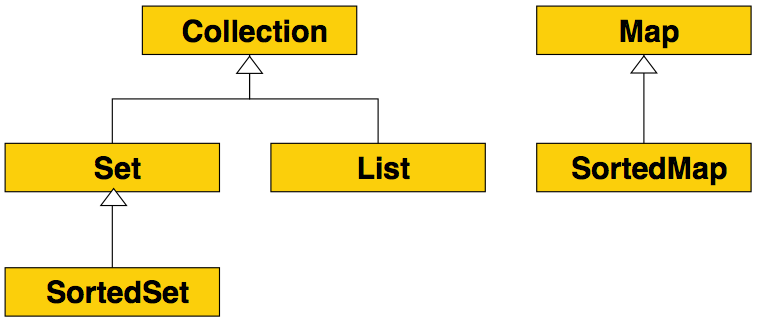
\includegraphics[scale=0.3]{jcf-interfaces.png}
\end{center}

\subsection{Der Iterator}
Ein Iterator ist immer zwischen zwei Elemente. Es gibt also in einer Collection mit n Elementen, n + 1 m�gliche Positionen an denen der Iterator stehen kann.
\lstinputlisting[language=java,caption=Iterator,style=JavaStyle]{iterator-interface.java}

\subsection{Die Implementierung}
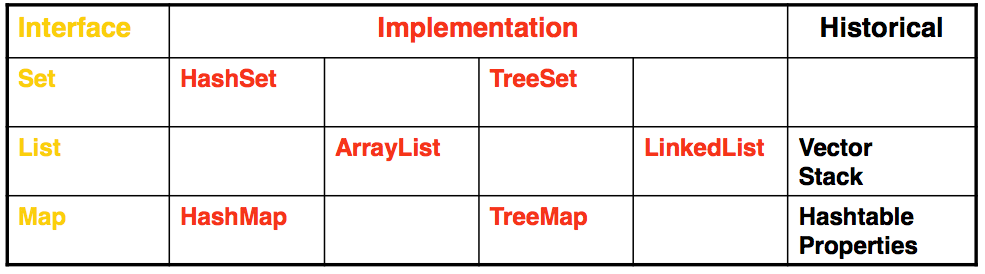
\includegraphics[scale=0.46]{jcf-implementations.png} 
\begin{description}
	\item[ArrayList] \hfill \\ Eine Implementierung welche ein Array darstellt bei dem man die Gr�sse ver�ndern kann.
	\item[LinkedList] \hfill \\ Eine doppelt verkettete Liste.
	\item[HashSet] \hfill \\ Die Elemente werden in einer Hash-Tabelle gespeichert.
	\item[TreeSet] \hfill \\ Die Elemente werden in einer Baumstruktur gespeichert.
	\item[Maps] \hfill \\ Eine Map ist wie ein W�rterbuch aufgebaut. Jeder Eintrag besteht aus einem Schl�ssel (key) und dem zugeh�rigen Wert (value). Jeder Schl�ssel darf in einer Map nur genau einmal vorhanden sein.
\end{description}
Wenn eine Klasse ein Interface implementiert, m�ssen immer alle Funktionen des Interface implementiert werden. In einer abstrakten Collection-Klasse k�nnen alle Funktionen bis auf zwei realisiert werden. F�r das Hinzuf�gen und f�r den Iterator ben�tigt es Kentnisse �ber die Datenstruktur. Hier das ein Beispiel einer Abstrakten Klasse:
\lstinputlisting[language=java,caption=Abstract Collection,style=JavaStyle]{abstract-collection.java}

\newpage
\section{Design Pattern}
Entwurfsmuster (englisch design patterns) sind bew�hrte L�sungsschablonen f�r wiederkehrende Entwurfsprobleme sowohl in der Architektur als auch in der Softwarearchitektur und -entwicklung. Sie stellen damit eine wiederverwendbare Vorlage zur Probleml�sung dar, die in einem bestimmten Zusammenhang einsetzbar ist.

\subsection{Types of Patterns}
\begin{description}
	\item[Software Pattern] \hfill
		\begin{itemize}
			\item Architectural Pattern (system design)
			\item Design Pattern (micro architectures)
			\item Coding Pattern / Idioms (low level)
		\end{itemize}
	\item[Analysis Pattern] \hfill
		\begin{itemize}
			\item Recurring \& reusable analysis models used in requirements engineering
		\end{itemize}
	\item[Organizational Patterns] \hfill
		\begin{itemize}
			\item Structure of organizations \& projects: XP, SCRUM
		\end{itemize}
	\item[Domain-Specific patterns] \hfill
		\begin{itemize}
			\item UI patterns, security patterns
		\end{itemize}
	\item[Anti-Patterns] \hfill
		\begin{itemize}
			\item Refactoring
		\end{itemize}
\end{description}

\subsection{Pattern Classification}

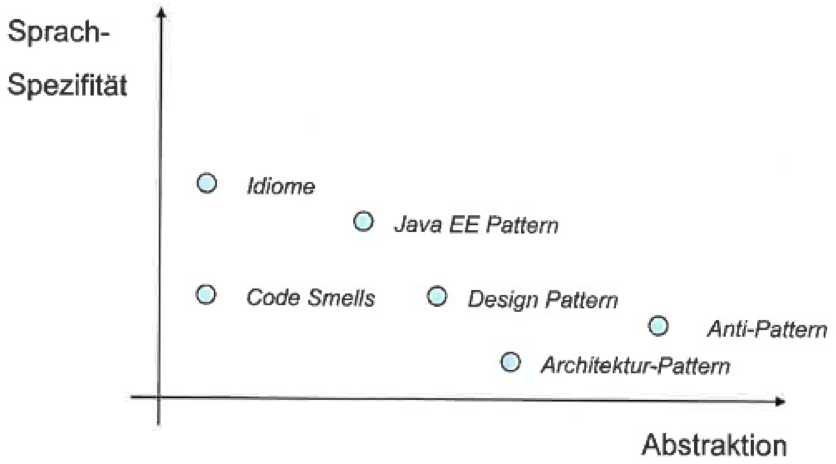
\includegraphics[scale=0.5]{pattern-classification.png}

\newpage
\section{Observer Pattern}
Also Known As \textbf{Publish-Subscribe} or \textbf{Listener Pattern}.

\subsection{Ziel}
\begin{itemize}
	\item 1:*-Relation between objects which allows to inform the dependent objects about state changes
	\item Consistency assurance between cooperating objects without connecting them too much
	\item Notification of a dependent object without knowing it
\end{itemize}

\subsection{Motivation}
\begin{center}
	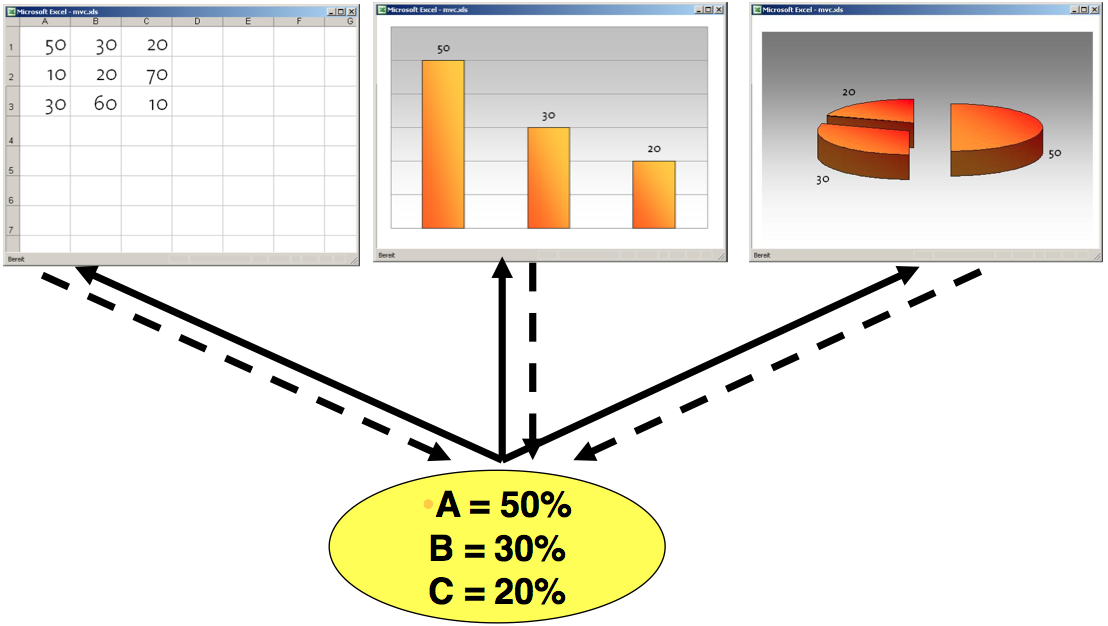
\includegraphics[scale=0.4]{observer-motivation.png}
\end{center}

\subsection{Struktur}
\begin{center}
	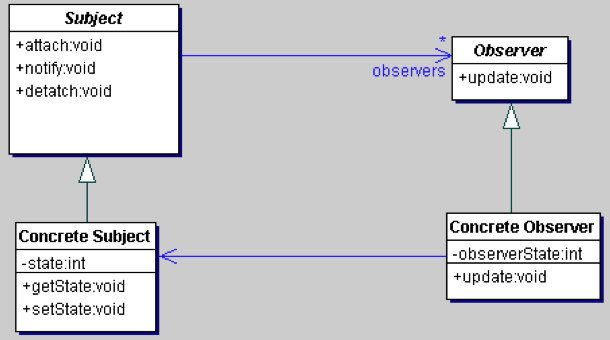
\includegraphics[scale=0.9]{observer-structure.png}
\end{center}

\subsection{Beispiel}
\lstinputlisting[language=java,caption=Beispiel Observer Pattern,style=JavaStyle]{observer.java}

\newpage
\section{State Pattern}

\subsection{Ziel}
Die Auslagerung von zustandsspezifischem Verhalten in einer Klasse. Erm�glicht mit dem Wechsel des Zustandes eines Objektes auch leicht das Verhalten zu �ndern.

\subsection{Motivation}
Die View des Grafikeditors hat eine Referenz auf ein abstraktes Tool-Interface. Diese Referenz definiert:
\begin{itemize}
	\item[a.] Der aktuelle Zeichenmodus
	\item[b.] Verhalten wenn Maus gedr�ckt wird
\end{itemize}

\subsection{Struktur}
Das zustandsabh�ngige Verhalten des Objekts wird in separate Klassen ausgelagert, wobei f�r jeden m�glichen Zustand eine eigene Klasse eingef�hrt wird, die das Verhalten des Objekts in diesem Zustand definiert. Damit der Kontext die separaten Zustandsklassen einheitlich behandeln kann, wird eine gemeinsame Abstrahierung dieser Klassen definiert. Bei einem Zustands�bergang tauscht der Kontext das von ihm verwendete Zustandsobjekt aus.
\begin{center}
	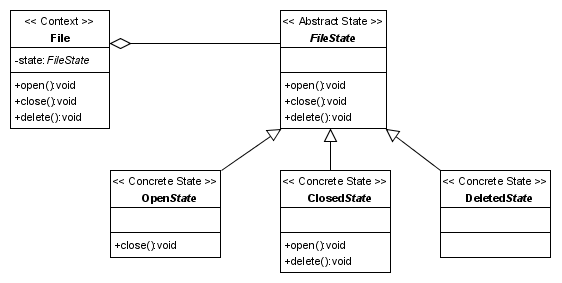
\includegraphics[scale=0.6]{state-structure.png}
\end{center}

\subsection{Beispiel}
\lstinputlisting[language=java,caption=Beispiel State Pattern,style=JavaStyle]{state.java}

\newpage
\section{Strategy Pattern}

\subsection{Ziel}
Eine Familie von Algorithmen definieren, von dem restlichen Programmcode abtrennen. Diese erm�glicht die Auswahl aus verschiedenen Implementierungen und dadurch erh�ht sich die Flexibilit�t und die Wiederverwendbarkeit.


\subsection{Struktur}
\begin{center}
	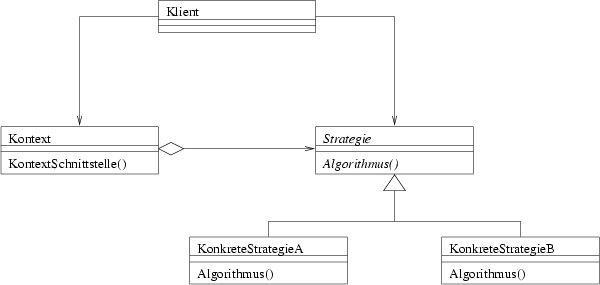
\includegraphics[scale=0.7]{strategy-structure.png}
\end{center}

\subsection{Beispiel}
\lstinputlisting[language=java,caption=Beispiel Strategy Pattern,style=JavaStyle]{strategy.java}

\newpage
\section{Null Object Pattern}

\subsection{Beschreibung}
Das Entwurfsmuster Nullobjekt findet Anwendung bei der Deaktivierung von Referenzen auf Variablen und besteht darin, der Referenz ein Objekt zuzuweisen, das keine Aktion ausf�hrt, anstatt die Referenz zu invalidieren. Dadurch wird erreicht, dass die Referenz auf die Variable zu jedem Zeitpunkt auf ein g�ltiges Objekt verweist, was Behandlungen von Sonderf�llen (das Nichtvorhandensein) er�brigt.

\subsection{Beispiel}
\lstinputlisting[language=java,caption=Beispiel Null Object Pattern,style=JavaStyle]{null.java}

% Inhalt Ende
\end{document}